% Geometry, font
\documentclass[12pt, letter]{article}
\usepackage[margin=0.8in]{geometry}
\usepackage[T1]{fontenc}
\usepackage{fourier}
\usepackage{titling}
\setlength{\droptitle}{-5em} 
\usepackage[parfill]{parskip}
\usepackage{graphicx}
\graphicspath{{imgs/}}
\usepackage{hyperref}

% Math stuff
\usepackage{amssymb}
\usepackage{amsmath}
\usepackage{bm}

% Code Highlighting
\usepackage{minted}
\usemintedstyle{solarizedlight}

\author{Zach Neveu}
\title{ Day 26 Notes }

\begin{document}
\maketitle
\section{Agenda}%
\label{sec:agenda}

\begin{itemize}
	\item Solving min-cost flow
	\item Cycle cancelling algorithm
\end{itemize}

\section{Min-Cost Flow}%
\label{sec:min_cost_flow}
\begin{itemize}
	\item Max-Flow can determine if given flow is viable
	\item Goal once this is found is to change it to minimize cost.
\end{itemize}

\section{Cycle-Cancelling Algorithm}%
\label{sec:cycle_cancelling_algorithm}
\begin{itemize}
	\item Use FF to find a max flow
	\item If it's too small, no flow exists
	\item While a net-negative cycle exists in the residual flow network, augment the flow around the cycle.
	\item When no negative-cycles exist, the flow has optimal cost.
\end{itemize}

\section{Application of Network Flow}%
\label{sec:application_of_network_flow}

\subsection*{Baseball Elimination}
\begin{itemize}
	\item 4 baseball teams trying to finish the season in first place.
	\item Win-Records:
	\begin{itemize}
		\item NY: 92 wins
		\item Boston: 90 wins
		\item Baltimore: 91 wins
		\item Toronto: 91 wins
	\end{itemize}
	\item Question: Can Boston get the most wins allowing for ties?
	\item Games remaining
	\begin{itemize}
		\item NY-Ba
		\item NY-To
		\item Ba-To
		\item Ba-Bo
		\item To-Bo
	\end{itemize}
	\item Manual Answer: Boston can't win: NY has to lose both of their games. This means that To and Ba each have one win, then they play each other so one of them will end up with 93 wins.
	\item Looking at fig. \ref{fig:bb} this makes sense, as there are only 2 units going to the sink and 3 coming from the source. This isn't feasible.
	\begin{figure}[h]
		\centering
		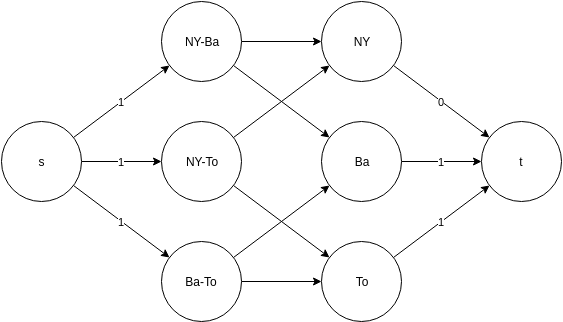
\includegraphics[width=0.8\textwidth]{bb}
		\caption{Baseball Games Flow Network}
		\label{fig:bb}
	\end{figure}
	\item Second (more complicated) example
	\item NY: 90, Ba: 88, To: 87, Bo: 79
	\item Remaining Games
	\begin{itemize}
		\item Ny-Bo: x4
		\item Ba-Bo: x4
		\item To-Bo: x4
		\item Ba-NY: x1
		\item Ba-To: x1
		\item NY-To: x6
	\end{itemize}
	\begin{figure}[h]
		\centering
		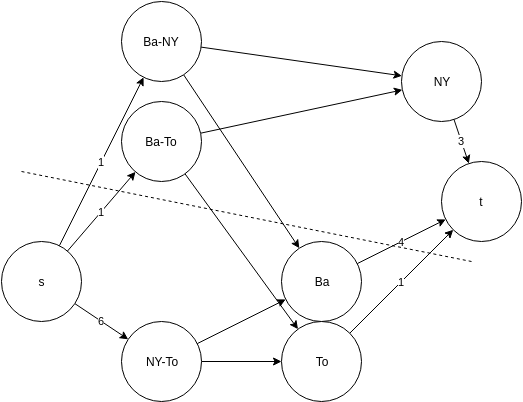
\includegraphics[width=0.8\textwidth]{bb2}
		\caption{Harder Magic Number Problem}
		\label{fig:bb2}
	\end{figure}
	\item Looking at fig. \ref{fig:bb2}, the maximum cut is 7. Boston needs 8 games to win, so they cannot do it.
\end{itemize}

\section{Hopping Airplane}%
\label{sec:hopping_airplane}
\begin{itemize}
	\item Goes to a bunch of sequential destinations, people get on and off at each destination.
	\item Every person starts at one city and ends at another.
	\item This makes $b[i,j]$ people who want to go from city i to city j (b)
	\item Each person pays a fair $f[i,j]$ to go from i to j (cost)
	\item Each plain has a capacity $p$
	\item Goal: maximize revenue
	\item Each city gets a node.
	\begin{figure}[h]
		\centering
		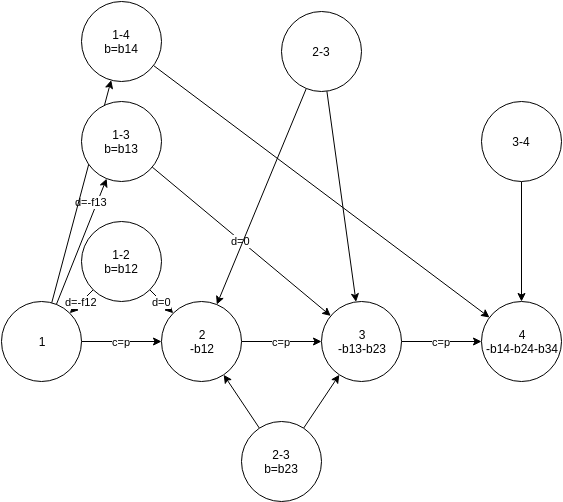
\includegraphics[width=0.8\textwidth]{airplane}
		\caption{Hopping Airplane Example}
		\label{fig:airplane}
	\end{figure}

\end{itemize}

\end{document}
